\section{Ruteo}

Realice el ruteo del siguiente programa e indique qué es lo que imprime. Cada vez que el valor de una variable cambie, escríbalo en una nueva fila de la tabla. Recuerde que si una variable es de tipo string, coloque su valor entre comillas simples ´  ´.
\textit{\textbf{Importante:} La tabla tiene suficientes filas.}

\begin{figure}[H]
    \centering
    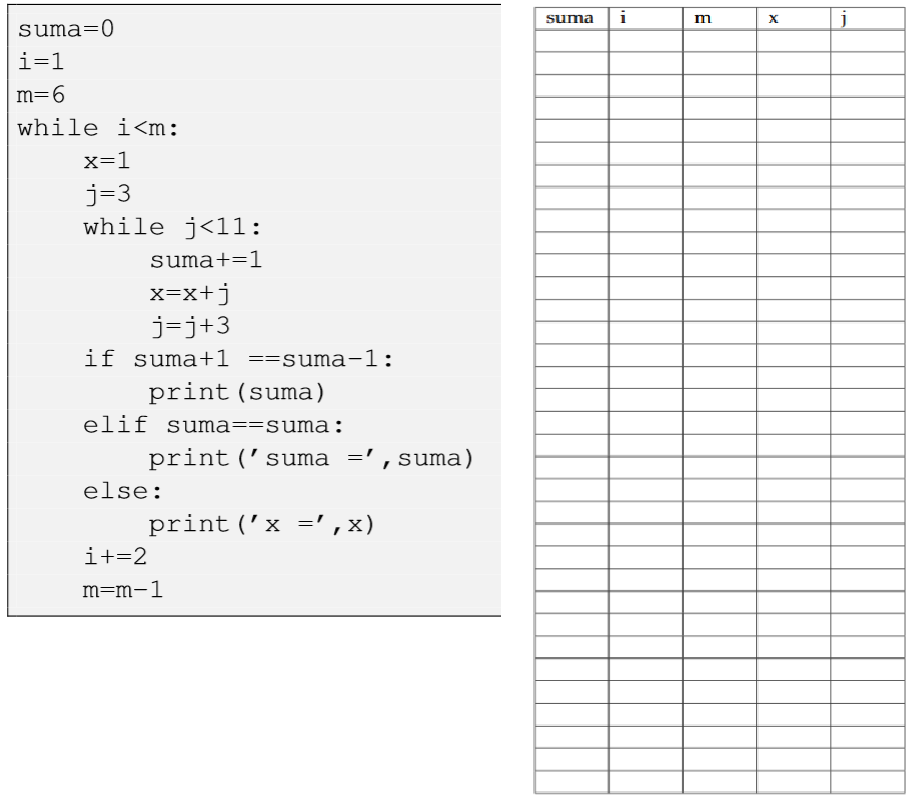
\includegraphics[width=\textwidth]{Guia/ruteo.png}
\end{figure}

Indique a continuación lo que imprime el programa